\chapter{Tez Çalışmasında Kullanılan Araçlar ve Cihazlar}

Bu çalışmada hedef cihazın, kablosuz ağ üzerinde programlanması ve veri aktarınımı sağlamak amacıyla sunucu cihaz olarak, Esp8266 mikrodenetleyicisi kullanılmıştır.
Hedef cihaz ile, sunucu cihaz arasında iletişimi sağlayan \acrfull{SWD} protokolünün işleyişini çözümlemek ve sunucu cihaz için yazılan kodların test sırasında işlemleri
incelemek amacıyla Lojik Analizör kullmılmıştır.

Hedef cihaz olarak ST firmasının ürettiği geliştirme kartı olan Discovery ailesinden, STM32F072 geliştirme kartı şeçilmiştir.

\section{ESP8266 Mikrodenetleyicisi}

ESP8266, Espressif firmasının geliştirdiği  mikrodenetleyicidir. Esp8266; 32 bitlik Tensilica mimarisine sahip işlemci, genel amaçlı çevre birimleri,
RF balun, güç amplifikatör devreleri, düşük gürültülü amplifikatör devreleri, filtreler ve güç yönetim modullerini küçük bir entegre paket halinde sunmaktadır. Aynı zamanda, 2.4 GHz Wi-Fi (802.11 b/g/n),
16 adet genel amaçlı giriş çıkış portu, \acrfull{I2C} portu, \acrfull{SPI} portu, 10 bitlik \acrfull{ADC}, 80 KiB  RAM mevcuttur. Harici olarak 8 MB'ta kadar SPI flash hafıza birimi
kullanılabilmektedir.


\begin{figure}[h]
\centering
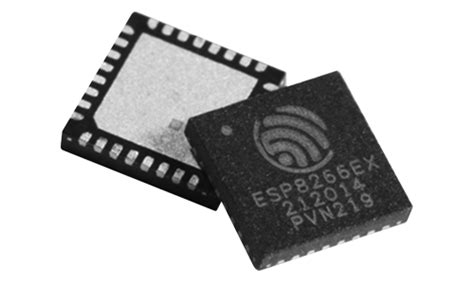
\includegraphics[width=\textwidth]{gorseller/esp8266ex}
\caption{ESP8266 Mikrodenetleyicisi.}\label{fig:esp8266ex}
\end{figure}

Geliştirme ortamı olarak, ESP8266 işlemcisi için kodların yazımında text editör olan VIM ve yazılan kodların derlenmesi, ESP8266 aktarılması için Arduino \acrfull{IDE}'si kullanılmıştır.
Espressif firmasının ESP8266 denetleyicisi için oluşturduğu \acrfull{SDK}, derleme zorluklarından ve derleme süreçlerinin uzun sürmesinden olayı Arduino IDE tercih edilmiştir.

ESP8266 denetleyicisi, hem SWD protokolü için sunucu cihaz hem de kullanıcı arayüzü olarak HTTP server olarak çalışacaktır. Kullanıcı arayüzünün platformdan ve işletim sisteminden bağımsız olması ve kurulum gerektirmediği için HTML ile web sayfası olarak tasarlanmıştır.

\section{Lojik Analizör}

Lojik analizör sayısal veri yolu üzerindeki işaretlerin gözlemlenmesi, ikilik tabanda oluşan kodları çözümlenmesini sağlayan mantıksal cihazdır. Bu çalışmada kullanılan lojik analizör Şekil \ref{fig:lojikAna}'de verilmiştir.

\begin{figure}[h]
\centering
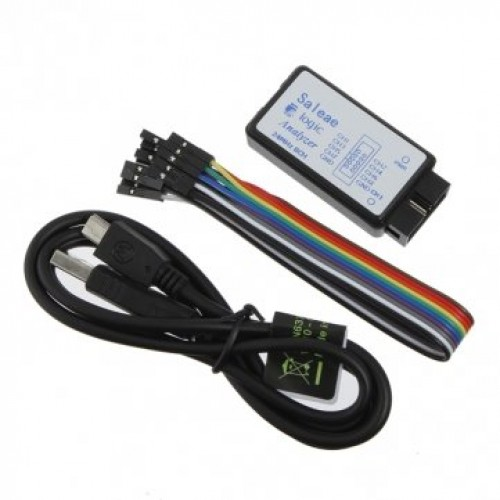
\includegraphics[width=0.7\textwidth]{gorseller/lojikAna}
\caption{Çalışmada Kullanılan Lojik Analizör}\label{fig:lojikAna}
\end{figure}

SWD protokolünü çözümlemek ve işlem sırasını çıkartmak için lojik analijör kullanılmıştır. Hedef cihaz olarak seçilen STM32F072 Discovery kartı üzerinde bulunan ST-Link SWD programlayıcısının, denetleyiciyi programlama sırasında lojik analizör ile protokol verilerini kaydederek protokol çözümlemesi yapıldı. Lojik analizörün arayüzünde dahili olarak bulunan SWD çözümleyici ile sistemin çalışması kontrol edildi.

\begin{figure}[h]
\centering
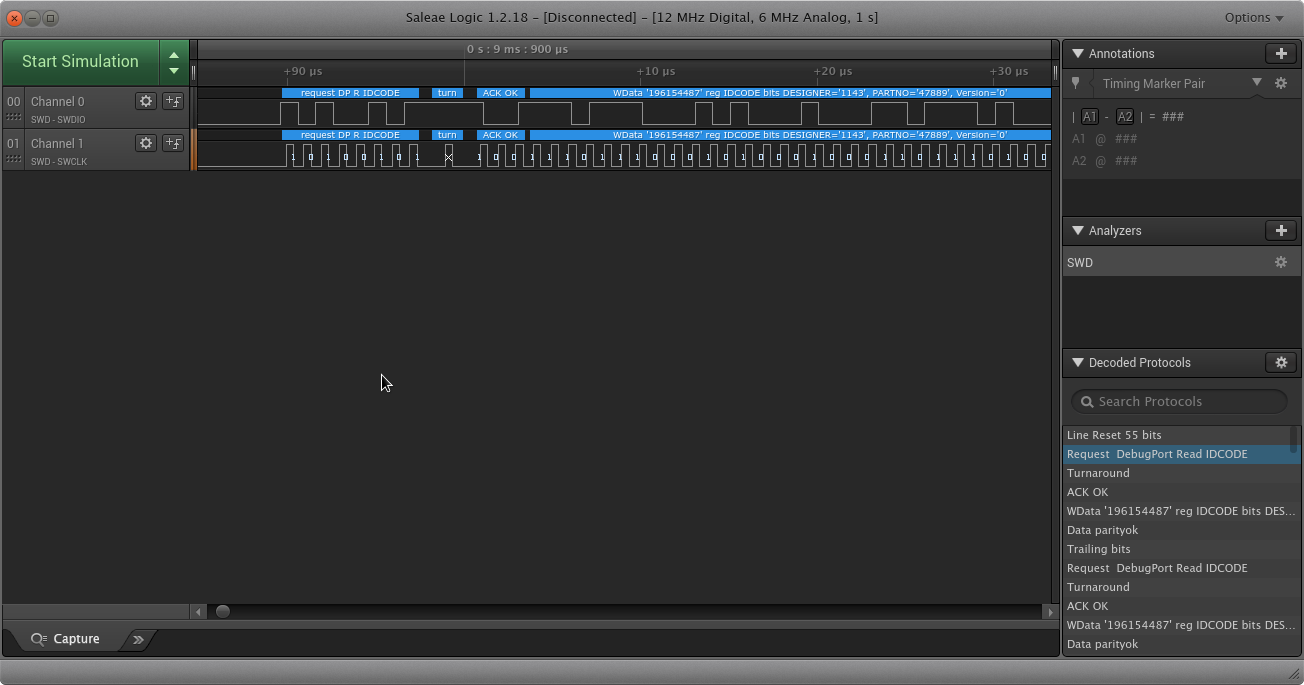
\includegraphics[width=\textwidth]{gorseller/lojikOut}
\caption{Örnek Lojik Analizör Çıktısı}\label{fig:lojikOut}
\end{figure}


Protokolün ve ardışık işlemlerin tanımlanması sonucunda, ESP8266 ile yapılan SWD uygulamasının testi sırasında lojik analizör kullanıldı.

\section{STM32F072 Discovery Kartı}

Elektronik ve yarıiletken komponent üreticisi olan STMicroelectronics tarafıdan geliştirilen, ARM Cortex-M0 mikroişlemcisine sahip olan STM32F072 mikrodenetleyicisi hedef cihaz olarak seçilmiştir. Ancak ARM tarafıdan geliştirilen SW-DP ve SWD, çoğu ARM işlemciler için ortak olduğu için bu tez çalışması için seçilen hedef cihaz dışında diğer ARM tabanlı mikrodenetleyiler bu çalışma kapsamı içindedir.

\begin{figure}[h]
\centering
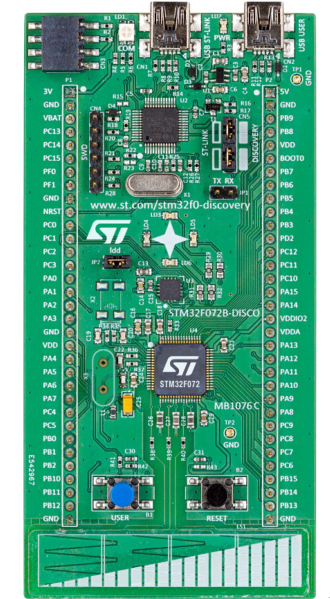
\includegraphics[width=0.4\textwidth]{gorseller/stmDisco}
\caption{STM32F072 Discovery Geliştirme Kartı.}\label{fig:stmDisco}
\end{figure}

STM32F0 Discovery kartı üzerinde, STM32F072RBT6 mikrodenetleyicisi, ST firmasının geliştirdiği jiroskop, liner dokumatik sensörü, buton, LED ve ST-LINK/V2 bulunmaktadır. STM32F072 kartı için test kodu; ST firmasının geliştirdiği STM32CUBEMX paket programı ile sistem konfigürasyon kodları oluşturulup, 'arm-none-eabi-gcc' derleyicisi ile derlenme işlemi yapılmıştır. Test kodu, STM32F072 Discovery kartı üzerinde bulunan 4 tane ledin yanıp sönmesi üzerine yazılmıştır. Farklı sıra ve süre ile oluşturulmuş test yazılımlar, sunucu cihazın programlayıcı özelliğinin test sırasında kullanılacaktır.



